\subsection{Descripci\'on del problema}

Se nos pide resolver el problema de obtener un orden de fabricaci\'on de joyas tal que se minimice la p\'erdida de dinero. Para lograr esto, se sabe que cada joya $j_{i}$ posee un tiempo de fabricaci\'on $t_{i}$ y un valor de devaluaci\'on diario $d_{i}$. \\

Para calcular la p\'erdida dado un orden de fabricaci\'on, se debe calcular la siguiente f\'ormula:

$\sum\limits_{i=0}^n d_{i}*dia\_finalizacion\_joya_{i}$

Donde $n$ es la cantidad de joyas menos uno, y $dia\_finalizacion\_joya_{i}$ es el dia global en el que se termina de fabricar la joya.\\

Por ejemplo, dadas las joyas $j_{0}$, $j_{1}$ y $j_{2}$ con tiempos de fabricaci\'on 3, 5 y 8, y valor de devaluaci\'on 10, 30 y 15 respectivamente, la soluci\'on \'optima ser\'ia el siguiente orden de fabricaci\'on:

\begin{center}
\begin{figure}[h]
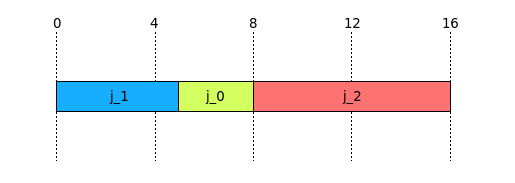
\includegraphics[scale=0.7]{./img/ej2_chart1.png}
\caption{Distribuci\'on de las joyas a fabricar}
\end{figure}
\end{center}

Esta disposici\'on se calcula con la siguiente formula:

$d_{0}*8 + d_{1}*5 + d_{2}*16 = 470$

Se puede comprobar calculando la misma formula para todas las permutaciones posibles del problema que esta es la \'optima: \\

$d_{0}*8 + d_{1}*5 + d_{2}*16 = 470$ \\
$d_{0}*16 + d_{1}*5 + d_{2}*13 +  = 505$ \\
$d_{0}*3 + d_{1}*8 + d_{2}*16 = 510$ \\
$d_{0}*16 + d_{1}*13 + d_{2}*8 = 670$ \\
$d_{0}*3 + d_{1}*16 + d_{2}*11 = 675$ \\
$d_{0}*11 + d_{1}*16 + d_{2}*8 = 710$ \\


\subsection{Resoluci\'on}

Para resolver el problema se decidio elegir algun tipo de medida de $peso$ para poder clasificar las joyas, donde $peso$ refiere especificamente a la siguiente ecuaci\'on: \\

$peso\_j_{i} = \frac{d_{i}}{t_{i}}$

Esta formula entrega el costo de fabricaci\'on por dia de cada joya. Luego el algoritmo procede a ordenar la fabricaci\'on de las joyas por costo por dia de mayor a menor. \\

Una descripci\'on del algoritmo en pseudo codigo:

\begin{itemize}
\item Para cada joya, calcular la relacion devaluacion sobre tiempo de la joya
\item Ordenar las joyas segun su costo por dia
\end{itemize}

\subsection{Demostraci\'on de la resoluci\'on}



\subsection{Complejidad del algoritmo}

Analizaremos a continuaci\'on la complejidad del algoritmo propuesto utilizando el pseudo c\'odigo como gu\'ia.

\begin{itemize}
\item para cada  joya en input, $O(n)$
\begin{itemize}
\item poner joya.porcentaje\_peso = joya.devaluacion / joya.tiempo\_fabricacion
\end{itemize}

\item ordenar joyas de mayor a menor por joya.porcentaje\_peso , $O(n*log(n))$
\end{itemize}


Notar que n es la cantidad de trabajos/joyas a confeccionar y que se simplific\'o el algoritmo para que fuera m\'as simple ver la complejidad.

Como se puede ver en el seguimiento, la complejidad del algoritmo elegido es O(n*log(n)) ya que es la complejidad predominante.\\

\subsection{Codigo fuente}

\lstset{language=C++,
                basicstyle=\ttfamily\footnotesize,
                keywordstyle=\color{blue}\ttfamily,
                stringstyle=\color{red}\ttfamily,
                commentstyle=\color{green}\ttfamily,
                morecomment=[l][\color{magenta}]{\#},
                breaklines=true
}
\begin{lstlisting}
               
typedef long double PorcentajePeso;

struct Joya {
	int identificador;
	int tiempo_fabricacion;
	int devaluacion_diaria;
	PorcentajePeso porcentaje_peso;
};

void resolver(list<Joya>& l){
	
	// Calculo la relacion entre la devaluacion diaria y el tiempo de cada joya : O(n)
	int i = 1;
	for(list<Joya>::iterator joya = l.begin(); joya != l.end(); joya++){
		
		joya->porcentaje_peso = ((PorcentajePeso) joya->devaluacion_diaria) / ((PorcentajePeso) joya->tiempo_fabricacion);
		joya->identificador = i; // La posicion en la lista original
		
		i++;
	}
	
	// Ordeno la lista de resultados segun el % de peso de mayor a menor: : O(n*log(n)) 
	// http://www.cplusplus.com/reference/list/list/sort/
	l.sort(pairCompare);

}
\end{lstlisting}

\subsection{Casos de prueba}

Se incluye entre los adjuntos el archivo TP:/ej2/casos\_borde.txt donde se detallan los siguientes casos posibles, en el mismo orden de aparici\'on:

\begin{itemize}
\item Un encargo de trabajo donde todas las joyas tienen el mismo valor de devaluaci\'on diario y el mismo tiempo de fabricaci\'on. Siguiendo la l\'ogica de nuestro algoritmo, se va a devolver un orden arbitrario pero cualquier orden es \'optimo en este caso.
\item Un encargo donde las diferencias son minimas, llegando casi al limite de presici\'on de la arquitectura.
\item Un caso con una \'unica soluci\'on posible
\end{itemize}

Se puede observar ejecutando el programa TP:/ej2/ej2 enviando como input el archivo mencionado que estos casos son resueltos correctamente.

\subsection{Performance}

Fueron generados casos de test aleateorios con el ejecutable TP:/ej2/test, que toma como parametro una semilla para el generador de n\'umeros pseudo aleatorios y luego el programa genera una determinada cantidad de listados de trabajos con un numero de joyas y valores al azar.\\

Para los casos "Datos aleatorios" fueron generadas 50 ejecuciones en cada una, ingresando como par\'ametro los n\'umeros de semilla 2 y 3. Estas ejecuciones tienen un numero de joyas al azar entre 1 y 1.000.000

Consideramos que no era apropiado evaluar casos bordes ya que, seg\'un se vi\'o en la secci\'on de Complejidad del algoritmo, recorremos la lista, realizamos operaciones y luego la ordenamos. Este algoritmo de sorting esta acotado por O(n*log(n)) a\'un considerando peores casos.

\begin{center}
\begin{figure}[h]
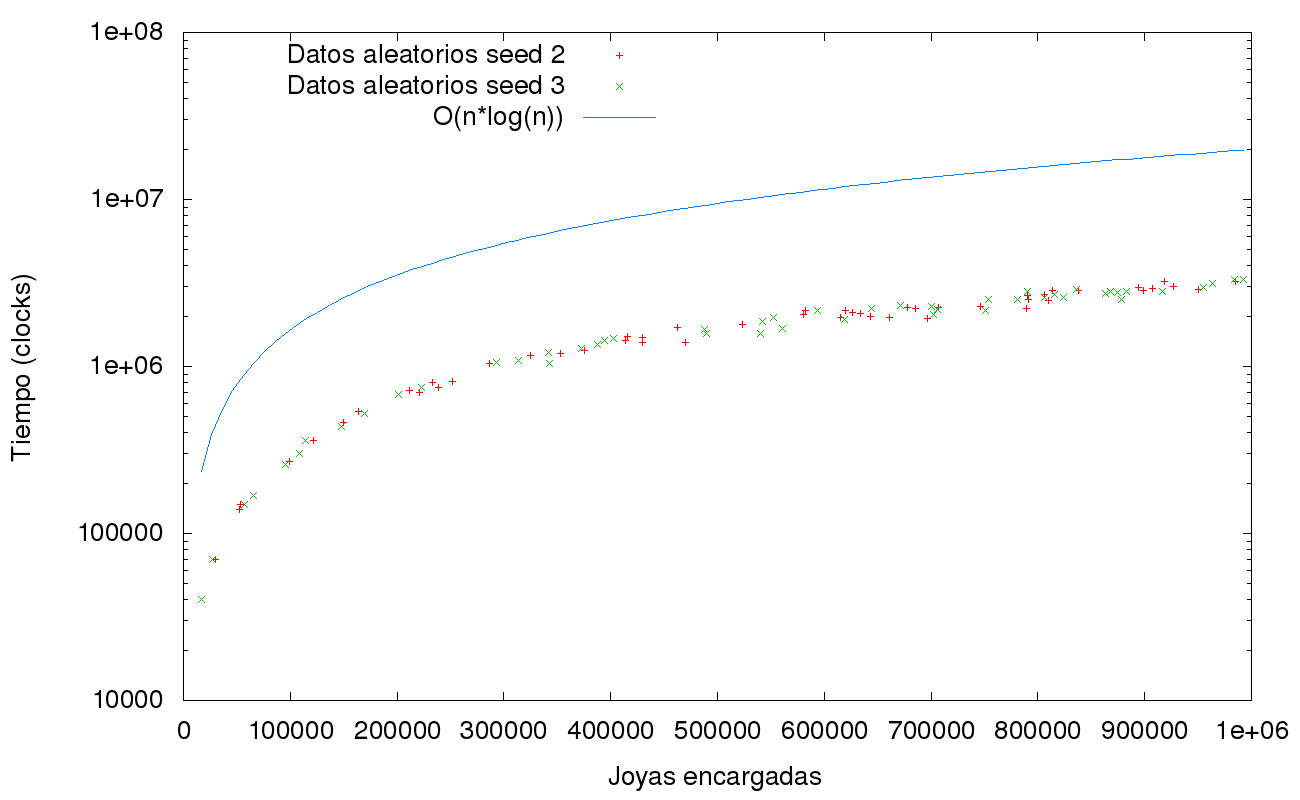
\includegraphics[scale=0.4]{./img/ej2_chart2.png}
\caption{Tiempo transcurrido por encargos de joyas}
\end{figure}
\end{center}

Como se puede observar el algoritmo corre en tiempos de ejecuci\'on bastante inferiores a la cota m\'axima propuesta por la c\'atedra de $O(n^2)$, a partir de un $n_{0}$
